\chapter{Detailed Results}
\label{ap:tabelas}

This appendix complements Chapter~\ref{cap:resultados} with the detailed results
of the feature selection scenario per percentile of features kept. All values are
produced by the script \texttt{tcc/scripts/gerar\_tabelas\_figuras.py} from the
raw result files available in the project repository.

\begin{table}[htb]
\centering
\caption{Effect of leakage in the feature selection scenario, per percentile and algorithm.}
\label{tab:alg-percentil}
\small
\setlength{\tabcolsep}{3pt}
\begin{tabular}{llrrrrrrrr}
\toprule
\textbf{perc} & \textbf{Alg.} & \multicolumn{3}{c}{\textbf{$\Delta R^2$ per data set}} & \textbf{$\Delta$RMSE (\%)} & \textbf{Better} & \textbf{Tie} & \textbf{Worse} & \textbf{$p_{\text{Holm}}$} \\
\cmidrule(lr){3-5}
& & Mean & Median & Max & Mean & (\%) & (\%) & (\%) & ($R^2$) \\
\midrule
1\% & LR & 0.0002 & 0.0000 & 0.0032 & 0.01 & 0.8 & 99.2 & 0.0 & 1.000 \\
1\% & KNN & $6.7\times10^{-5}$ & 0.0000 & 0.0014 & 0.00 & 0.8 & 98.4 & 0.8 & 1.000 \\
1\% & DT & -0.0015 & 0.0000 & 0.0000 & -0.05 & 0.0 & 99.2 & 0.8 & 1.000 \\
1\% & RF & -0.0004 & 0.0000 & 0.0000 & -0.02 & 0.0 & 99.2 & 0.8 & 1.000 \\
1\% & SVR & $-6.1\times10^{-5}$ & 0.0000 & $7.4\times10^{-17}$ & -0.00 & 0.0 & 99.2 & 0.8 & 1.000 \\
\midrule
5\% & LR & 0.0002 & 0.0000 & 0.0032 & 0.01 & 0.8 & 99.2 & 0.0 & 1.000 \\
5\% & KNN & 0.0001 & 0.0000 & 0.0016 & 0.01 & 6.3 & 89.7 & 4.0 & 1.000 \\
5\% & DT & -0.0015 & 0.0000 & 0.0000 & -0.05 & 0.0 & 99.2 & 0.8 & 1.000 \\
5\% & RF & -0.0004 & 0.0000 & 0.0000 & -0.02 & 0.0 & 99.2 & 0.8 & 1.000 \\
5\% & SVR & $-6.1\times10^{-5}$ & 0.0000 & $5.6\times10^{-17}$ & -0.00 & 0.0 & 99.2 & 0.8 & 1.000 \\
\midrule
10\% & LR & 0.0083 & 0.0000 & 0.1816 & 0.57 & 6.3 & 92.1 & 1.6 & 1.000 \\
10\% & KNN & 0.0078 & 0.0000 & 0.0886 & 0.57 & 11.1 & 76.2 & 12.7 & 1.000 \\
10\% & DT & 0.0093 & 0.0000 & 0.0974 & 0.65 & 6.3 & 92.1 & 1.6 & 0.721 \\
10\% & RF & 0.0075 & 0.0000 & 0.1483 & 0.57 & 6.3 & 92.1 & 1.6 & 0.820 \\
10\% & SVR & 0.0076 & 0.0000 & 0.1680 & 0.56 & 6.3 & 92.1 & 1.6 & 0.721 \\
\midrule
20\% & LR & 0.0293 & 0.0000 & 0.6181 & 0.64 & 4.0 & 92.9 & 3.2 & 1.000 \\
20\% & KNN & 0.0046 & 0.0000 & 0.1717 & 0.27 & 15.1 & 73.8 & 11.1 & 1.000 \\
20\% & DT & -0.0072 & 0.0000 & 0.0121 & -0.16 & 3.2 & 92.9 & 4.0 & 1.000 \\
20\% & RF & 0.0004 & 0.0000 & 0.0687 & 0.04 & 3.2 & 92.9 & 4.0 & 1.000 \\
20\% & SVR & 0.0142 & $1.9\times10^{-17}$ & 0.3009 & 0.49 & 4.0 & 92.9 & 3.2 & 0.115 \\
\bottomrule
\end{tabular}

\\[2pt]
\footnotesize Source: The Author. Columns as in Table~\ref{tab:alg-normalizacao}; Holm adjustment applied within each percentile.
\end{table}

\begin{table}[htb]
\centering
\caption{Data set--algorithm combinations with the largest mean $\Delta R^2$ in the normalization scenario.}
\label{tab:top-normalizacao}
\small
\begin{tabular}{llrr}
\toprule
\textbf{Data set} & \textbf{Alg.} & \textbf{$\Delta R^2$} & \textbf{$\Delta$RMSE (\%)} \\
\midrule
542\_pollution & SVR & 0.0330 & 2.11 \\
542\_pollution & KNN & 0.0070 & 0.46 \\
560\_bodyfat & KNN & 0.0062 & 1.49 \\
1096\_FacultySalaries & KNN & 0.0046 & 1.03 \\
1089\_USCrime & SVR & 0.0032 & 0.32 \\
542\_pollution & RF & 0.0025 & 0.24 \\
1027\_ESL & DT & 0.0022 & 0.53 \\
574\_house\_16H & KNN & 0.0010 & 0.11 \\
\bottomrule
\end{tabular}

\\[2pt]
\footnotesize Source: The Author. Values averaged over repetitions.
\end{table}

\begin{table}[htb]
\centering
\caption{Data set--algorithm combinations with the largest mean $\Delta R^2$ in the imputation scenario.}
\label{tab:top-imputacao}
\small
\begin{tabular}{llrr}
\toprule
\textbf{Data set} & \textbf{Alg.} & \textbf{$\Delta R^2$} & \textbf{$\Delta$RMSE (\%)} \\
\midrule
1028\_SWD & DT & 0.0038 & 0.28 \\
542\_pollution & DT & 0.0036 & -0.21 \\
1089\_USCrime & LR & 0.0030 & 0.49 \\
542\_pollution & SVR & 0.0029 & 0.07 \\
1089\_USCrime & SVR & 0.0028 & 0.64 \\
1029\_LEV & SVR & 0.0023 & 0.24 \\
574\_house\_16H & DT & 0.0020 & 0.13 \\
1029\_LEV & LR & 0.0020 & 0.21 \\
\bottomrule
\end{tabular}

\\[2pt]
\footnotesize Source: The Author. Values averaged over imputers, missing rates, and repetitions.
\end{table}

\begin{figure}[htb]
\centering
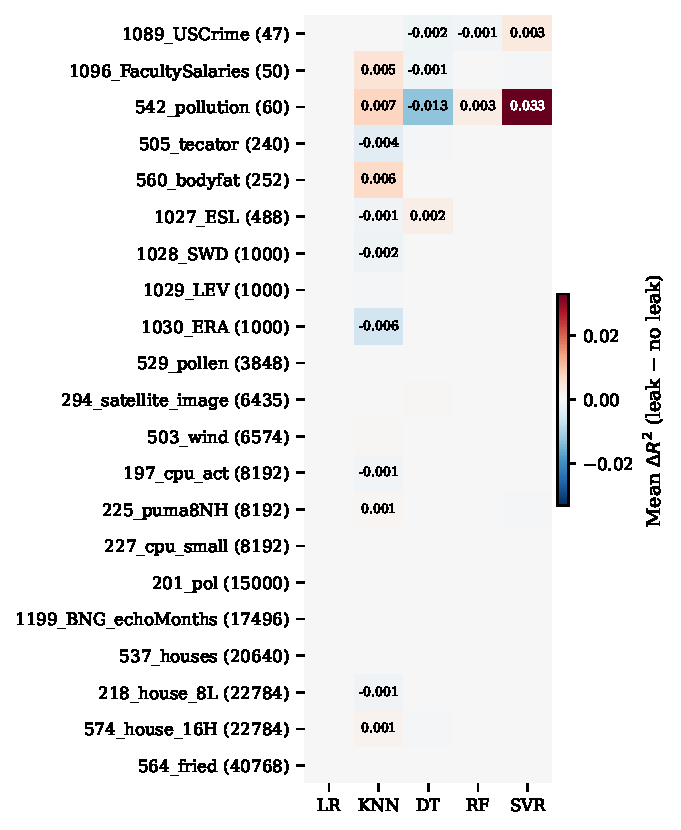
\includegraphics[width=0.75\textwidth]{figuras/fig_heatmap_normalization.pdf}
\caption{Mean $\Delta R^2$ per data set and algorithm in the normalization scenario.}
\label{fig:heatmap-normalizacao}
\legend{Source: The Author. Values below 0.0005 in absolute value are omitted.}
\end{figure}

\begin{figure}[htb]
\centering
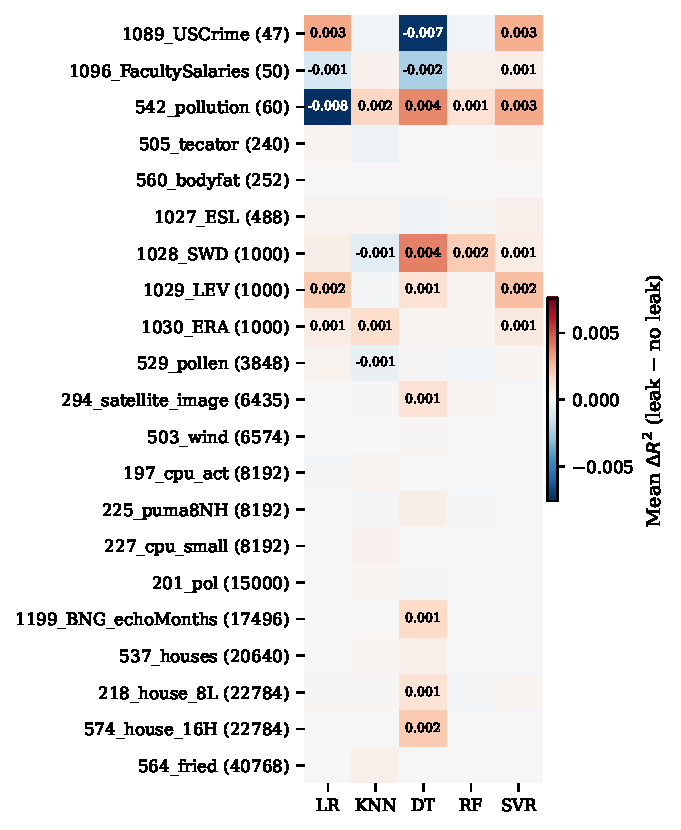
\includegraphics[width=0.75\textwidth]{figuras/fig_heatmap_imputation.pdf}
\caption{Mean $\Delta R^2$ per data set and algorithm in the imputation scenario.}
\label{fig:heatmap-imputacao}
\legend{Source: The Author. Values below 0.0005 in absolute value are omitted.}
\end{figure}
